\documentclass{a0poster}
\usepackage{fancytikzposter}

\usetemplate{3}

\usepackage[margin=\margin cm, paperwidth=84.1cm, paperheight=118.9cm]{geometry}

%% changing the fonts
\usepackage{cmbright}
%\usepackage[default]{cantarell}
%\usepackage{avant}
%\usepackage[math]{iwona}
\usepackage[math]{kurier}
\usepackage[T1]{fontenc}


\title{Diffusion-Controlled Reactions over Fluctuating Barriers}

\author{Jakob J. Kolb}


\begin{document}
\ClearShipoutPicture
\AddToShipoutPicture{\BackgroundPicture}

\noindent
\begin{tikzpicture}
    \initializesizeandshifts
    \titleblock{50}{1}
    \blocknode{Motivation}{
        ***Some sort of an Abstract***
    }
    \blocknode{System description}{
        \begin{minipage}[t]{.5 \textwidth}
            ***System description and sketch***
            have to figure out, how to fix the scalling issue with \textbackslash input
        \end{minipage}\begin{minipage}[t]{.5 \textwidth}
            \begin{tikzfigure}[Caption]
                %% Creator: Inkscape inkscape 0.48.4, www.inkscape.org
%% PDF/EPS/PS + LaTeX output extension by Johan Engelen, 2010
%% Accompanies image file 'Skizze.pdf' (pdf, eps, ps)
%%
%% To include the image in your LaTeX document, write
%%   \input{<filename>.pdf_tex}
%%  instead of
%%   \includegraphics{<filename>.pdf}
%% To scale the image, write
%%   \def\svgwidth{<desired width>}
%%   \input{<filename>.pdf_tex}
%%  instead of
%%   \includegraphics[width=<desired width>]{<filename>.pdf}
%%
%% Images with a different path to the parent latex file can
%% be accessed with the `import' package (which may need to be
%% installed) using
%%   \usepackage{import}
%% in the preamble, and then including the image with
%%   \import{<path to file>}{<filename>.pdf_tex}
%% Alternatively, one can specify
%%   \graphicspath{{<path to file>/}}
%% 
%% For more information, please see info/svg-inkscape on CTAN:
%%   http://tug.ctan.org/tex-archive/info/svg-inkscape
%%
\documentclass[
	ngerman,	%deutsch
	a4paper,	%A4 Format
	12pt,		%Schriftgröße
	twoside,		%zweiseitig
%	liststoto
%	bibtotocnumbered
				]{book}%Artikel
\usepackage[ansinew]{inputenc}	%Zeichenkodierung
\usepackage[T1]{fontenc}
\usepackage[english]{babel}			%deutsche Silbentrennung
\usepackage[english]{hyperref}
%\usepackage[sort&compress]{natbib}
\usepackage{
    textcomp,
    floatrow,
    color,
    cite,
	amsmath,
	amssymb,
        titleps,
%    libertine,
	amsfonts,		%Mathepakete
    graphicx,		%Bilder einbinden
	%a4wide,			%volle Seitenbreite
	multirow,		%Zellen verbinden in Tabellen
	booktabs,		%schöne Tabellen
	array,			%Arrays halt
	float,			%Gleitumgebungen genau HIER setzen
	caption,		%zusätzliche Optionen für Unterschriften
	fancyhdr,		%schöne Kopf-/Fußzeilen
	ragged2e,		%besseres Centering, RaggedRight und RaggedLeft
	caption,
	hhline,
	wrapfig,
        bbm,
    listings,
    bm
	}
\usepackage[toc,page]{appendix}
\usepackage{listings}
\usepackage{color}
\usepackage[margin=0.01 in]{geometry}


\begin{document}

\eject \pdfpagewidth=4in \pdfpageheight=3.5in

\begingroup%
  \makeatletter%
  \providecommand\color[2][]{%
    \errmessage{(Inkscape) Color is used for the text in Inkscape, but the package 'color.sty' is not loaded}%
    \renewcommand\color[2][]{}%
  }%
  \providecommand\transparent[1]{%
    \errmessage{(Inkscape) Transparency is used (non-zero) for the text in Inkscape, but the package 'transparent.sty' is not loaded}%
    \renewcommand\transparent[1]{}%
  }%
  \providecommand\rotatebox[2]{#2}%
  \ifx\svgwidth\undefined%
    \setlength{\unitlength}{240bp}%
    \ifx\svgscale\undefined%
      \relax%
    \else%
      \setlength{\unitlength}{\unitlength * \real{\svgscale}}%
    \fi%
  \else%
    \setlength{\unitlength}{\svgwidth}%
  \fi%
  \global\let\svgwidth\undefined%
  \global\let\svgscale\undefined%
  \makeatother%
 \begin{picture}(0,1)%

	
    \put(0,0){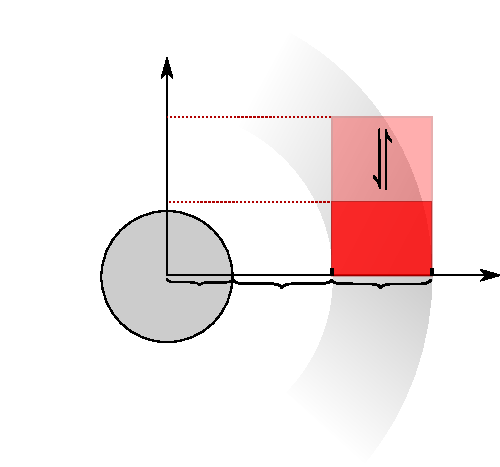
\includegraphics[width=\unitlength]{Skizze2.pdf}}%
    \put(0.21972941,0.78296832){\color[rgb]{0,0,0}\makebox(0,0)[lb]{\smash{$U(r)$}}}%
    \put(0.23700218,0.69336482){\color[rgb]{0,0,0}\makebox(0,0)[lb]{\smash{$U_1$}}}%
    \put(0.2447597,0.52890544){\color[rgb]{0,0,0}\makebox(0,0)[lb]{\smash{$U_0$}}}%
    \put(0.37532722,0.31427216){\color[rgb]{0,0,0}\makebox(0,0)[lb]{\smash{$R_s$}}}%
    \put(0.96482605,0.32743337){\color[rgb]{0,0,0}\makebox(0,0)[lb]{\smash{$r$}}}%
    \put(0.66943563,0.6095448){\color[rgb]{0,0,0}\makebox(0,0)[lb]{\smash{$W_{10}$}}}%
    \put(0.78814443,0.6107948){\color[rgb]{0,0,0}\makebox(0,0)[lb]{\smash{$W_{01}$}}}%
    \put(0.54834834,0.30763194){\color[rgb]{0,0,0}\makebox(0,0)[lb]{\smash{$l$}}}%
    \put(0.74263382,0.31010763){\color[rgb]{0,0,0}\makebox(0,0)[lb]{\smash{$gl$}}}%
    \put(0.63208542,0.40873922){\color[rgb]{0,0,0}\makebox(0,0)[lb]{\smash{$a$}}}%
    \put(0.87325729,0.40939026){\color[rgb]{0,0,0}\makebox(0,0)[lb]{\smash{$b$}}}%


    \end{picture}%
\endgroup%
\end{document}

            \end{tikzfigure}
        \end{minipage}
        
    }
    \blocknode{Analytical Tricks and stuff}{
        Lots of Formulas and explanations
    }
    \startsecondcolumn
    \blocknode{Density profiles}{
        \begin{minipage}[t]{.6 \textwidth}
        \begin{tikzfigure}[Caption]
            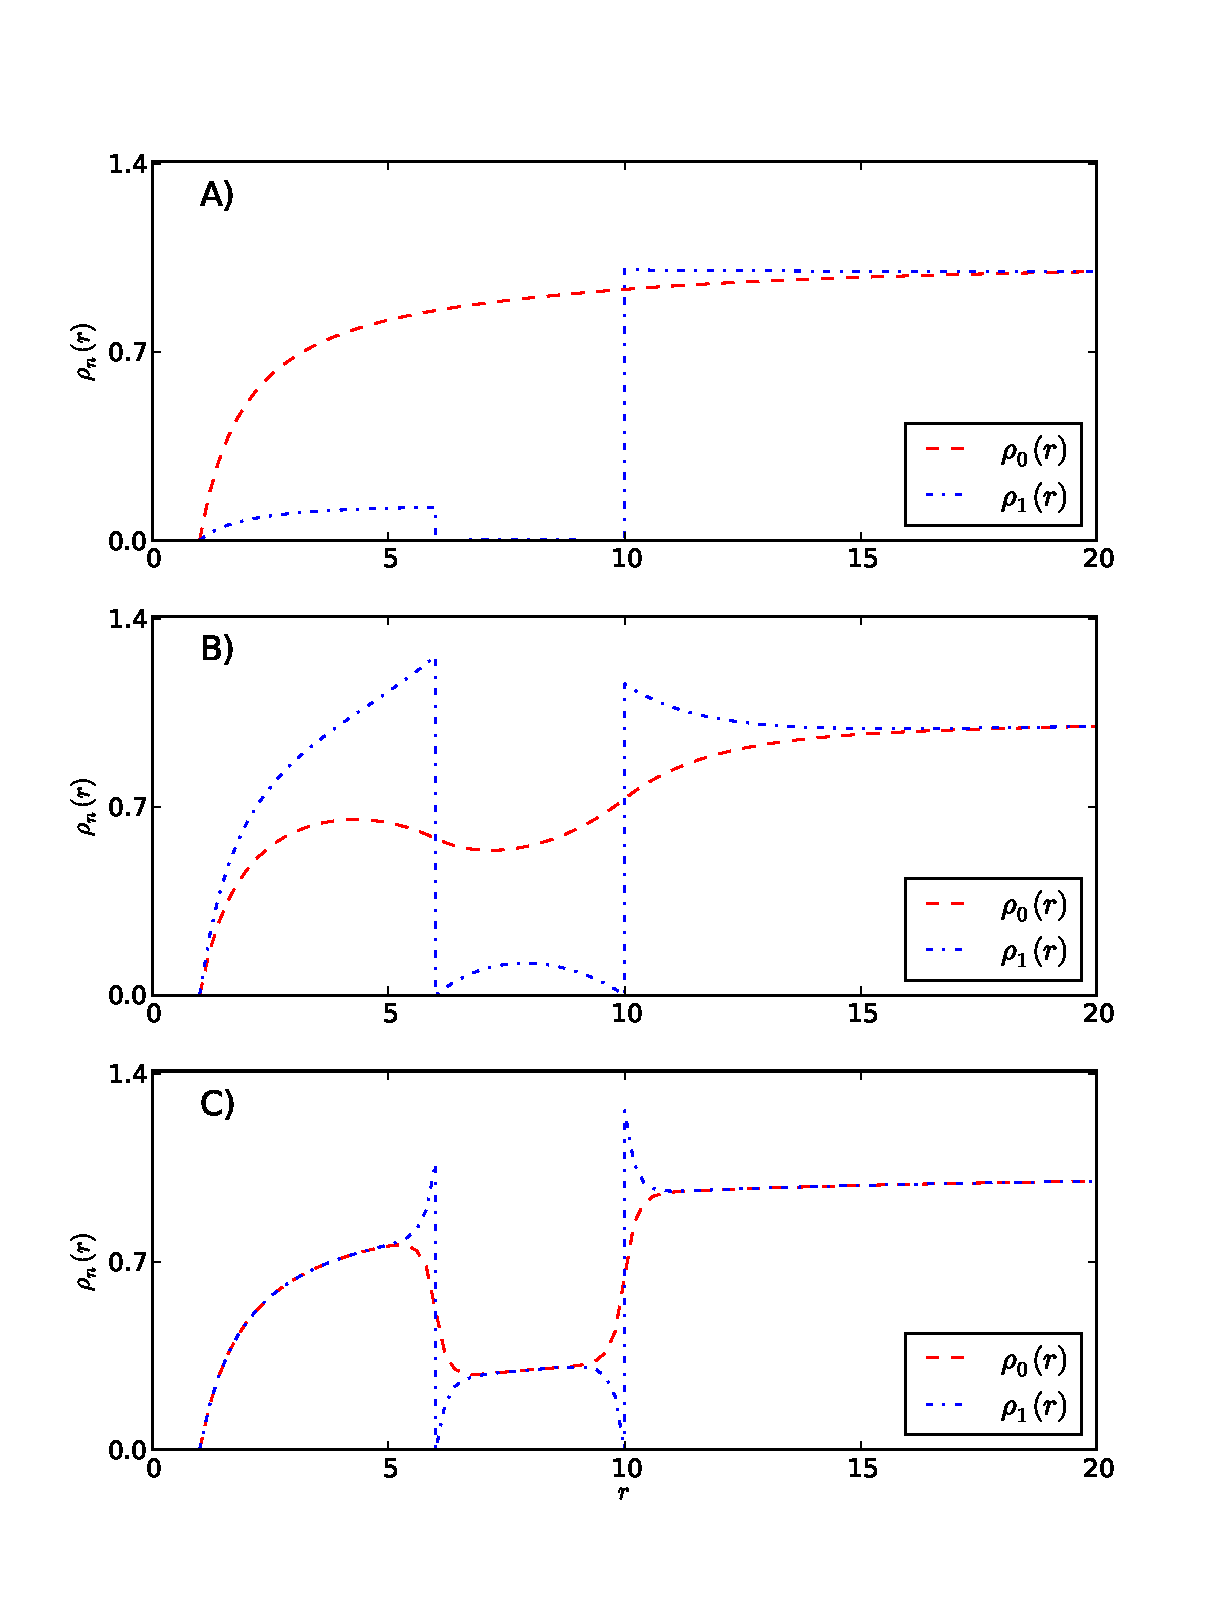
\includegraphics[width = 0.9\textwidth]{plots/density_profiles.pdf}
        \end{tikzfigure}
        \end{minipage}\begin{minipage}[t]{.4 \textwidth}
            just some text explaining the figure
        \end{minipage}
    }
    \blocknode{Absorption Rates}{
        \begin{minipage}[t]{.6 \textwidth}
             \begin{tikzfigure}[Caption]
                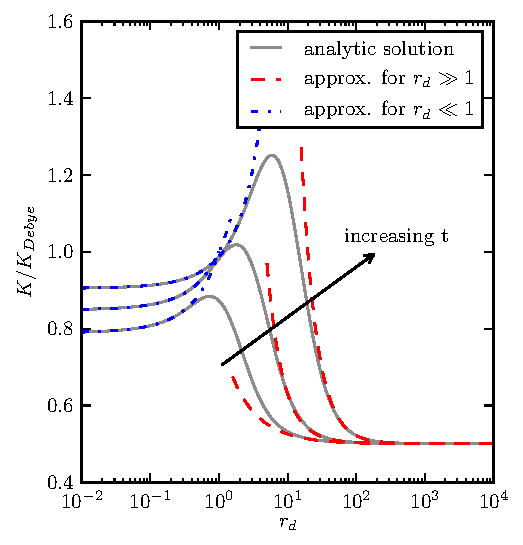
\includegraphics[width = 0.9 \textwidth]{plots/rep_barrier.pdf}
            \end{tikzfigure}
            \begin{tikzfigure}[Caption]
                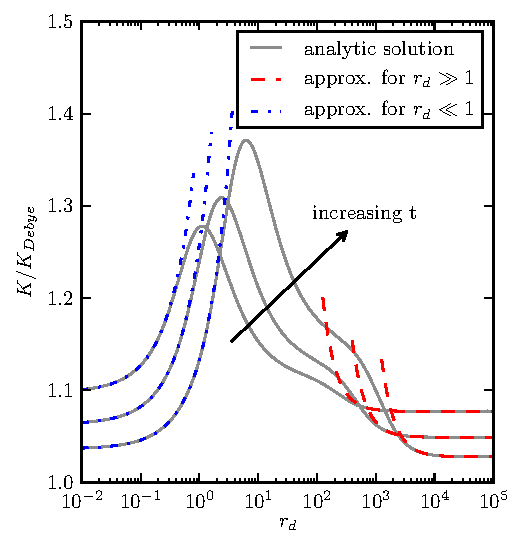
\includegraphics[width = 0.9 \textwidth]{plots/att_barrier.pdf}
            \end{tikzfigure}
        \end{minipage}\begin{minipage}[t]{.4 \textwidth}
            some more text explaining these figure and giving hints to resonant activation phenomena
        \end{minipage}


    }
\end{tikzpicture}
\end{document}
